\section{Introduction: Model-Native Computing Demands an Architecture}
\label{sec:intro}

Large language models are undergoing a fundamental transition, from a \emph{model technology} to a \emph{system technology}.
Starting with GPT-3's demonstration of in-context learning~\cite{brown2020gpt3}, through the LLaMA family's catalysis of open-weight ecosystems~\cite{llama2023}, and onward to the rapid proliferation of tool use~\cite{schick2023toolformer}, retrieval-augmented generation~\cite{lewis2020rag}, autonomous agents~\cite{yao2023react}, and code generation systems~\cite{openhands_paper_2025,sweagent2024}, the research frontier has shifted decisively.
The central question is no longer ``how do we train more capable models?'' but rather ``how do we organize intelligence into systems that are stable, scalable, and auditable?''

This shift is reshaping engineering practice itself.
The engineer's role is migrating from writing code line by line to orchestrating ensembles of specialized agents, compressing entire development cycles from weeks to hours~\cite{anthropic2026agenticreport}.
Yet many of the bottlenecks that now dominate practice (memory bandwidth walls~\cite{gholami2024memorywall}, cache reuse inefficiency~\cite{kwon2023pagedattention}, context management~\cite{memgpt2023}, batch scheduling~\cite{orca2022}, and sandboxed permission control~\cite{ironclaw2025}) are not failures of model capability.
They are, at their core, \emph{systems problems}.

The impact is already measurable in production.
Engineers at Rakuten used Claude Code to autonomously extract activation vectors from the vLLM codebase (12.5 million lines of code) in seven hours, achieving 99.9\% numerical accuracy.
An Augment Code enterprise customer delivered a project that their CTO had estimated at four to eight months in just two weeks~\cite{anthropic2026agenticreport}.
These are not laboratory demonstrations; they are evidence that the challenges of model-native computing have moved from theoretical possibility to engineering reality.

Given these parallels, a natural question arises: classical computer architecture solved a remarkably similar class of complexity-management problems through a mature stack of layered abstractions.
Can that intellectual framework transfer to model-native computing systems?

\subsection{A Natural Analogy}

The core mapping between the two worlds is summarized in Table~\ref{tab:analogy-mapping}.

\begin{table}[t]
\centering
\footnotesize
\caption{Core analogy mapping between classical computing and model-native computing.}
\label{tab:analogy-mapping}
\begin{tabularx}{\textwidth}{>{\raggedright\arraybackslash}p{0.28\textwidth}>{\raggedright\arraybackslash}p{0.28\textwidth}>{\raggedright\arraybackslash}p{0.34\textwidth}}
\toprule
\textbf{Classical Computing} & \textbf{Model-Native Computing} & \textbf{Shared Problem} \\
\midrule
CPU & LLM inference core & General-purpose computation \\
Cache (L1/L2/L3) & KV cache & Hot data reuse, memory optimization \\
Virtual memory & Context window + external memory & Finite-capacity address space mgmt \\
Operating system & Agent runtime & Scheduling, permissions, resource mgmt \\
I/O buses (PCIe/USB) & MCP / A2A protocols & Standardized peripheral/tool integration \\
Applications \& users & Agent apps \& domain experts & Turning computation into solutions \\
\bottomrule
\end{tabularx}
\end{table}

The correspondence runs deeper than surface resemblance.
(1)~The LLM inference core provides general-purpose semantic understanding and generation, much as a CPU executes a general instruction set, with different models (GPT-4, Claude, LLaMA) resembling different microarchitectures that implement the same ``instruction set'' of reasoning with distinct performance profiles.
(2)~The \emph{KV cache} reuses previously computed attention key-value pairs during autoregressive decoding to avoid redundant computation, mirroring exactly how a CPU cache exploits temporal locality to reuse hot data.
PagedAttention~\cite{kwon2023pagedattention} makes this analogy explicit, borrowing the operating system's paging mechanism to partition KV caches into fixed-size blocks allocated on demand.
(3)~The context window is strictly bounded (e.g., 128K tokens), yet agents routinely require access to knowledge and interaction histories far exceeding this limit---precisely the problem that motivated virtual memory.
MemGPT~\cite{memgpt2023} formalizes this as \emph{virtual context management}, directly analogous to the operating system's virtual memory abstraction.
(4)~Agent runtimes such as Codex~\cite{openai_codex_overview_2026}, Claude Code~\cite{anthropic_claudecode_overview_2026}, and OpenHands~\cite{openhands_paper_2025} manage task decomposition, tool dispatch, sub-agent coordination, sandbox isolation, and result submission: a responsibility envelope that increasingly resembles an operating system kernel.
(5)~MCP (Model Context Protocol)~\cite{mcp_intro_2026} defines a standardized interface between agents and external tools, while A2A (Agent-to-Agent Protocol)~\cite{google_a2a_2025} specifies interoperability contracts among agents.
Together they play the role of I/O buses: MCP functions as a vertical bus (analogous to PCIe, connecting an agent to its tools), while A2A functions as a horizontal interconnect (analogous to a network fabric, connecting agents to one another)~\cite{agentprotocols2025}.

In 2023, Andrej Karpathy captured this intuition in a single sentence: ``LLMs are not chatbots, they are the kernel process of a new Operating System''~\cite{karpathy2023llmos}.
The observation resonated widely precisely because it named something already happening: the engineering problems accumulating around large models look increasingly like classical computer systems problems.

\begin{figure}[t]
\centering
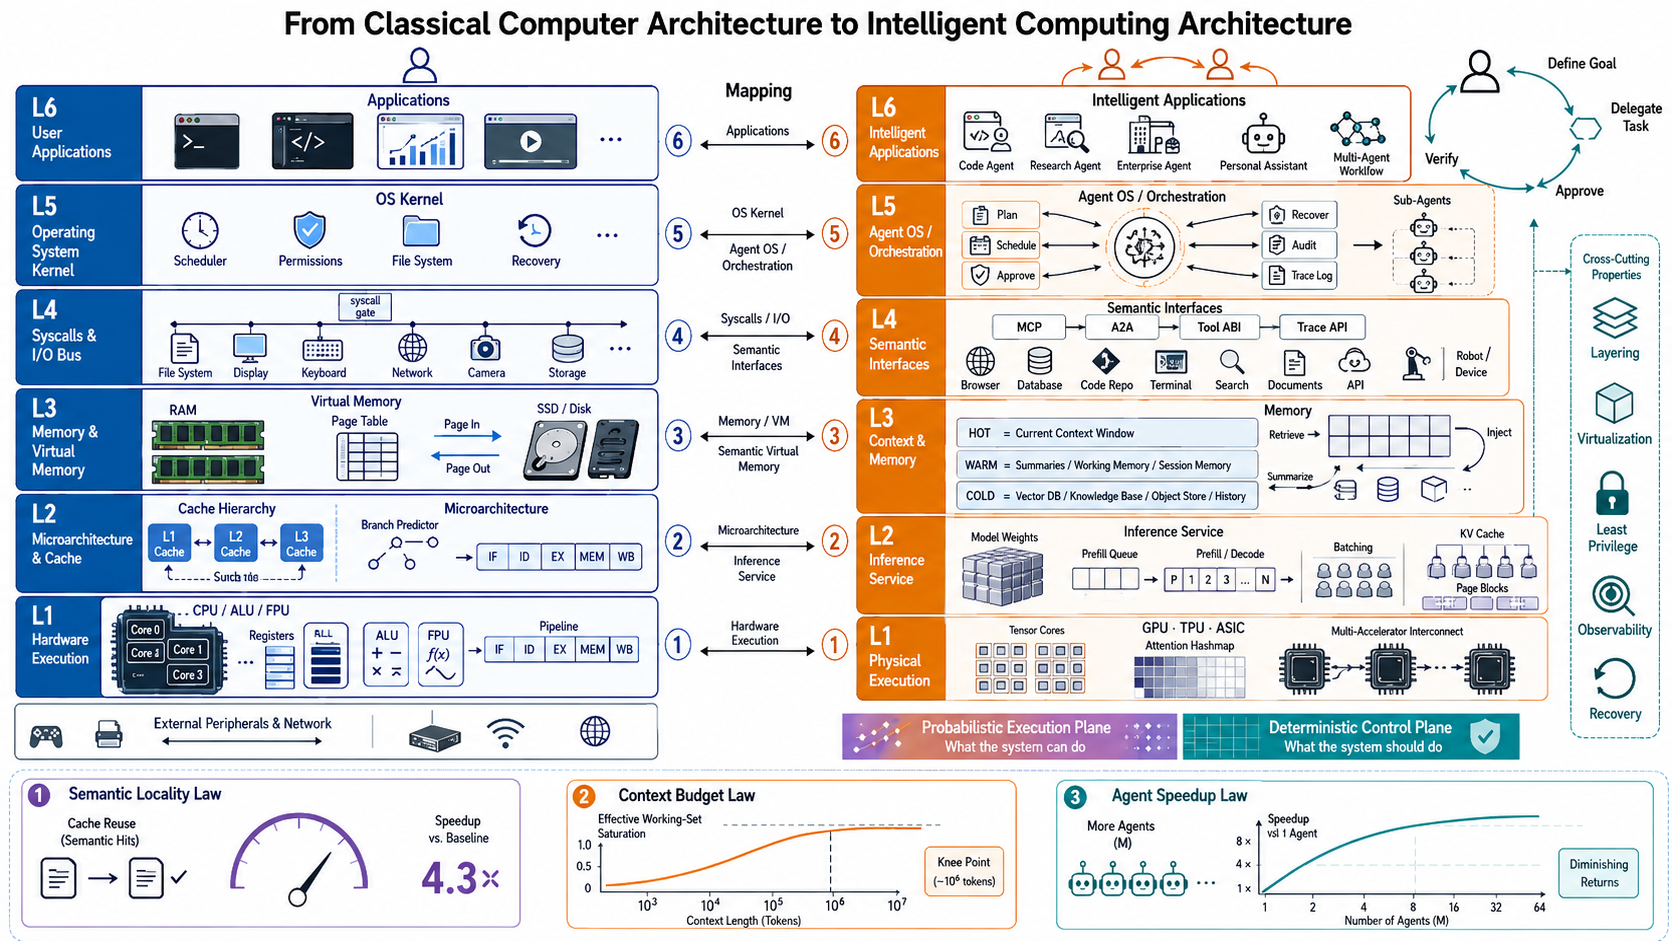
\includegraphics[width=0.98\textwidth]{figures/fig_analogy_map.png}
\caption{Overview analogy mapping between computer architecture and model-native computing systems}
\label{fig_analogy_map}
\end{figure}

\subsection{From Intuition to Problem}

An analogy, however, is not a theory.
``Resembles'' does not imply ``is.''
If the mapping remains at the level of rhetoric, it yields inspirational metaphors but not testable predictions or actionable design principles.

Multiple independent efforts have already explored facets of this analogy from different angles.
AIOS treats the LLM as an operating system kernel, building an agent runtime with a scheduler, context manager, and memory manager~\cite{mei2024aios}.
MemGPT~\cite{memgpt2023} applies virtual-memory thinking to context management.
Mi et al.\ design agent architectures by drawing on process models, file systems, and other classical abstractions~\cite{mi2025llmagentscomputersystems}.
Ge et al.\ articulate the vision of ``LLM as OS, Agents as Apps''~\cite{ge2023llmos}.
L2MAC frames the LLM as a stored-program automatic computer~\cite{holt2024l2mac}.
ArbiterOS defines the LLM as a ``Probabilistic CPU'' governed by a higher-level governor~\cite{arbiteros2025}.
AgentOS positions it as a reasoning kernel~\cite{agentos2025}.
MemOS elevates memory itself to a first-class operating-system resource~\cite{memos2025}.
On the inference engineering side, Mei et al.\ (2025) survey the emerging discipline of \emph{context engineering}, defining it as the systematic optimization of all information supplied to an LLM~\cite{contextengineer_survey2025}.

These works each cover one or several layers of the system stack---the OS layer, the memory layer, the agent kernel, the inference layer.
Yet they suffer from a fundamental \emph{metaphor conflict}: is the model a CPU, an OS kernel, or a reasoning kernel?
More critically, they lack a unified layered model, well-defined inter-layer interfaces, and quantifiable design principles.
Moreover, nearly all of them treat the human as a boundary condition of the system rather than as a core component of the interaction loop.
The latest industrial evidence, however, tells a different story: the collaboration pattern between human judgment and agent execution, not the agent's standalone capability, is the primary determinant of system effectiveness.
Engineers report using AI for approximately 60\% of their work, yet they can \emph{fully delegate} only 0--20\% of tasks~\cite{anthropic2026agenticreport}.
This is the collaboration paradox: AI is embedded deeply into the workflow, but meaningful autonomous delegation remains elusive.

The situation echoes the early days of computer architecture.
Before the introduction of the Instruction Set Architecture (ISA) as a contract between hardware and software, every new CPU required a complete rewrite of all software, and no improvement at one layer could be leveraged by another.
Without an analogous contract for model-native computing, each new system must be built from scratch, and insights remain siloed within individual projects.

\subsection{Contributions}

Accordingly, this paper makes five contributions.

\begin{enumerate}
\item We return to the foundational abstractions of computer architecture, operating systems, and distributed systems to distill an analogy framework suited to the model-native system stack, explicitly delineating where the analogy holds and where it breaks down.

\item We survey the landscape of related work, expose the metaphor conflicts among existing approaches, and propose the \textbf{dual-plane architecture} as a unifying resolution, partitioning the model-native stack into a \emph{probabilistic execution plane} (model inference and generation) and a \emph{deterministic control plane} (system scheduling and control), with clearly defined interfaces between the two.

\item Building on this foundation, we introduce the \textbf{Intelligent Computing Architecture (ICA)}: a six-layer framework with inter-layer interface contracts and six design axioms.

\item We propose three \textbf{quantitative laws} for model-native computing, aiming to serve the same foundational role that Amdahl's Law and the Roofline model play in classical computer architecture, and we validate them against published data.

\item We survey current open-source implementations and industrial practice, and we chart a research roadmap for the field.
\end{enumerate}
